% !TeX spellcheck = <none>
\documentclass[a4paper]{article}
%\usepackage[export]{adjustbox}
\usepackage[a4paper, total={6in, 8in}]{geometry}
\usepackage{amsmath, amssymb}
\usepackage{graphicx}
\usepackage{subfigure}
%\usepackage{pdfpages}
\usepackage{multirow}
%\usepackage{float}
%\usepackage{indentfirst}
%\setlength{\parindent}{2em}
%\usepackage{fancyhdr}
%\pagestyle{fancy}
%\usepackage{lastpage}
%\headheight 14pt
%\usepackage{float}
%\renewcommand\baselinestretch{1.2}

\title{Simple tests on iterative method with arclength parameterizing}
\author{Chen Ziheng}
\date{\today}

\begin{document}
\maketitle
\part{Test on a non-singular case}
\section{Arclength parameterization}
Consider the Hamiltonian of the following diffusion-driven system
\begin{equation}
	H = \frac{1}{2} \left \langle p, ap \right \rangle + \left \langle b, p \right \rangle .
\end{equation}
If we apply arclength parameterizing, we will have
\begin{align}
	\label{eqn:arclength-param}
	x' &= \frac{C}{|b|_a}(ap+b), \\
	p' &= -\frac{C}{|b|_a}(\nabla b)^T p ,
\end{align}
where $C$ denotes the full length of the solution $x$.
\section{An example}
To begin with, we check a trivial case: $a$ is identity, $b$ in the form of $-Bx$, and $B$ is normal for the time being.
Then the analytical solution is clear:
\begin{align}
	p(t) &= exp(B^T t) p_0, \\
	x(t) &= (B + B^T)^{-1} p(t),
\end{align}
here $t$ takes value from $[0, +\infty)$

First we give a non-singular border condition: $p(0) = (4, 1)^T$ and $x(1) = (0.9993063, 0)^T$.
The iterations terminates when the difference of adjacent two $p(1)$s is smaller than a given criterion.
\section{How to measure error}
Besides, we also need to measure how the solution differs from the analytic one; take $resolution=3, criterion=10^{-6}$ as an exmaple (Figure \ref{fig:p1-arclength-i8} and \ref{fig:p1-arclength-i15}).
\begin{figure}[h]
	\centering
	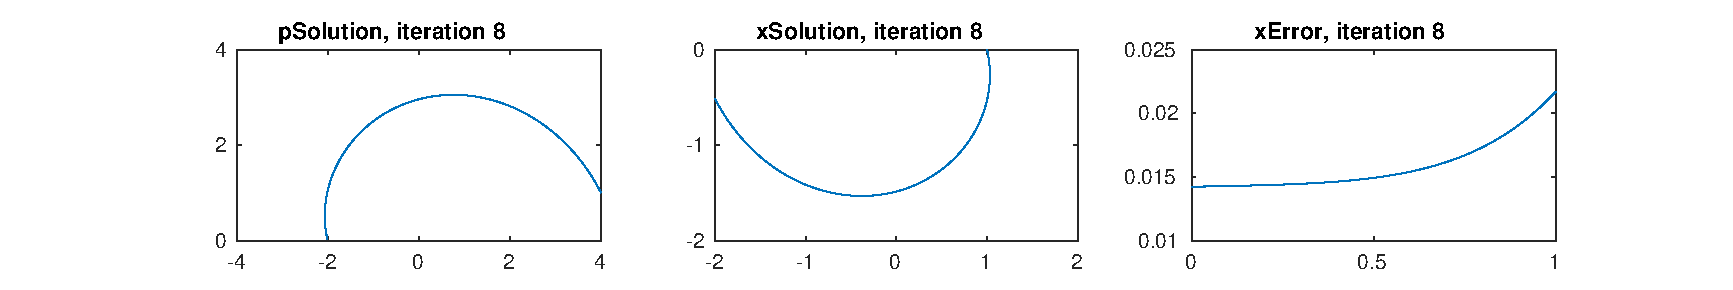
\includegraphics[width=\textwidth]{part1-arclength-iteration8}
	\caption{8th Iteration Result}
	\label{fig:p1-arclength-i8}
\end{figure}
\begin{figure}[h]
	\centering
	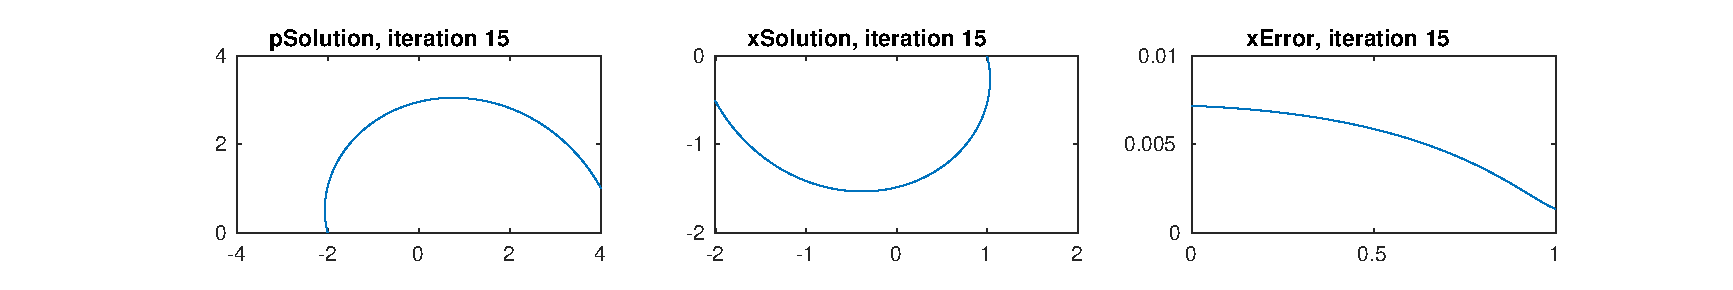
\includegraphics[width=\textwidth]{part1-arclength-iteration15}
	\caption{15th Iteration Result}
	\label{fig:p1-arclength-i15}
\end{figure}
In the first several iterations, the error mainly distributes around $t=1$; however, as the iterations going on, the error turns to gather around $t=0$, which is the ending point of the iteration process.
So we measure the difference where $t=0$ to estimate the whole error.
\section{Arclength-param result}
The following chart shows how the error descends under arclength method; the error is indeed in first order to the resolution (so as the time needed).
\begin{figure}[h]
	\centering
	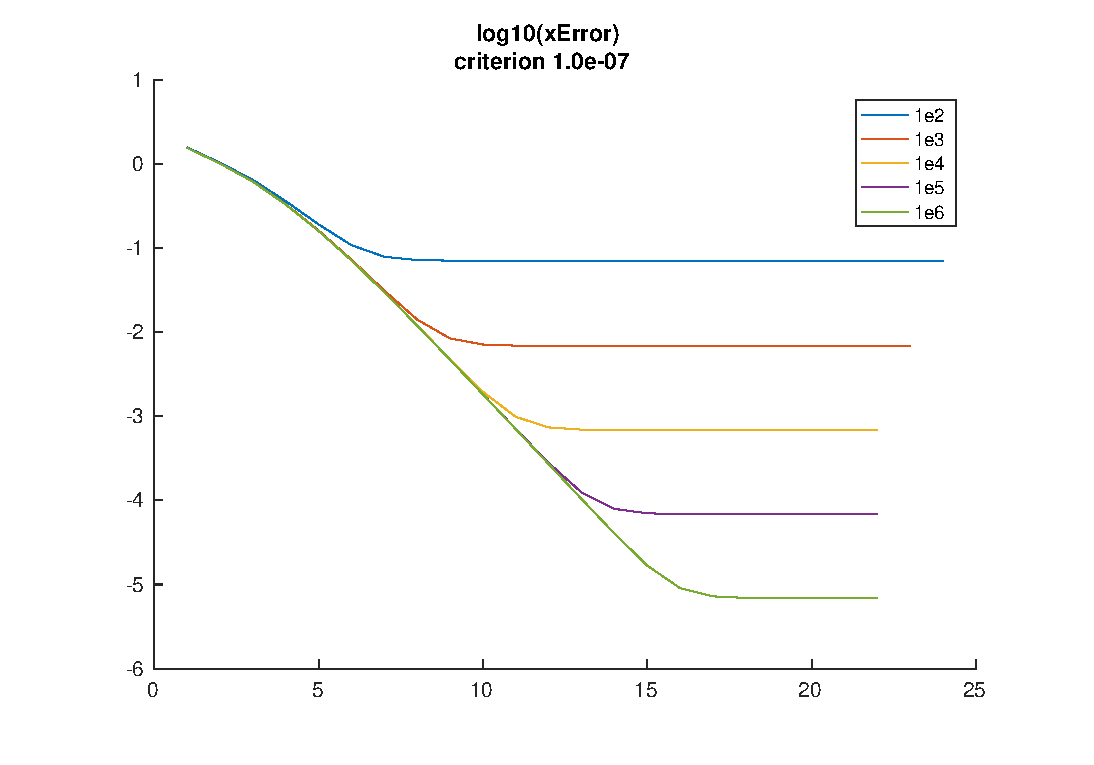
\includegraphics[width=\textwidth]{part1-arclength-resolution-error}
	\caption{Error of Arclength Parameterizing Method}
	\label{fig:p1-arclength-error}
\end{figure}

\emph{Note:} The precision is directly affected by the initial value.
If we take $x(1) = (1, 0)$ rather than that magic number, the iterative method fails to achieve the corresponding precision at the resolution of $10^4$ (for the fact that $1 - 0.9993063 > 10^{-4}$).
\section{Normal method result}
As for normal method, the result is quite boring: it converges after just two iterations!
But that cannot prove any point, since in this case $p$ only relies on itself
$$\frac{dp}{dt} = B^T p$$,
so the $p$ part is precise, which can hardly happen in more complex cases.

\part{Failure on a singular case}
\section{Arclength-param result}
If we change the border condition of the equations \eqref{eqn:arclength-param} to $p(0) = (4, 1)^T$ and $x(1) = (0, 0)^T$, the singularity of $\frac{dx}{ds}$ at $s=1 (x=0)$ will emerge immediately.
If we ignore the singulartiy for the time being, just taking any finite number as the derivative the singular point, the solution will diverge quickly, let alone converge at a first order speed.
So direct use of iterative method may be too reckless to get a working effect.
\\
The following chart shows the failure even at the first iterative round.
\begin{figure}[h]
	\centering
	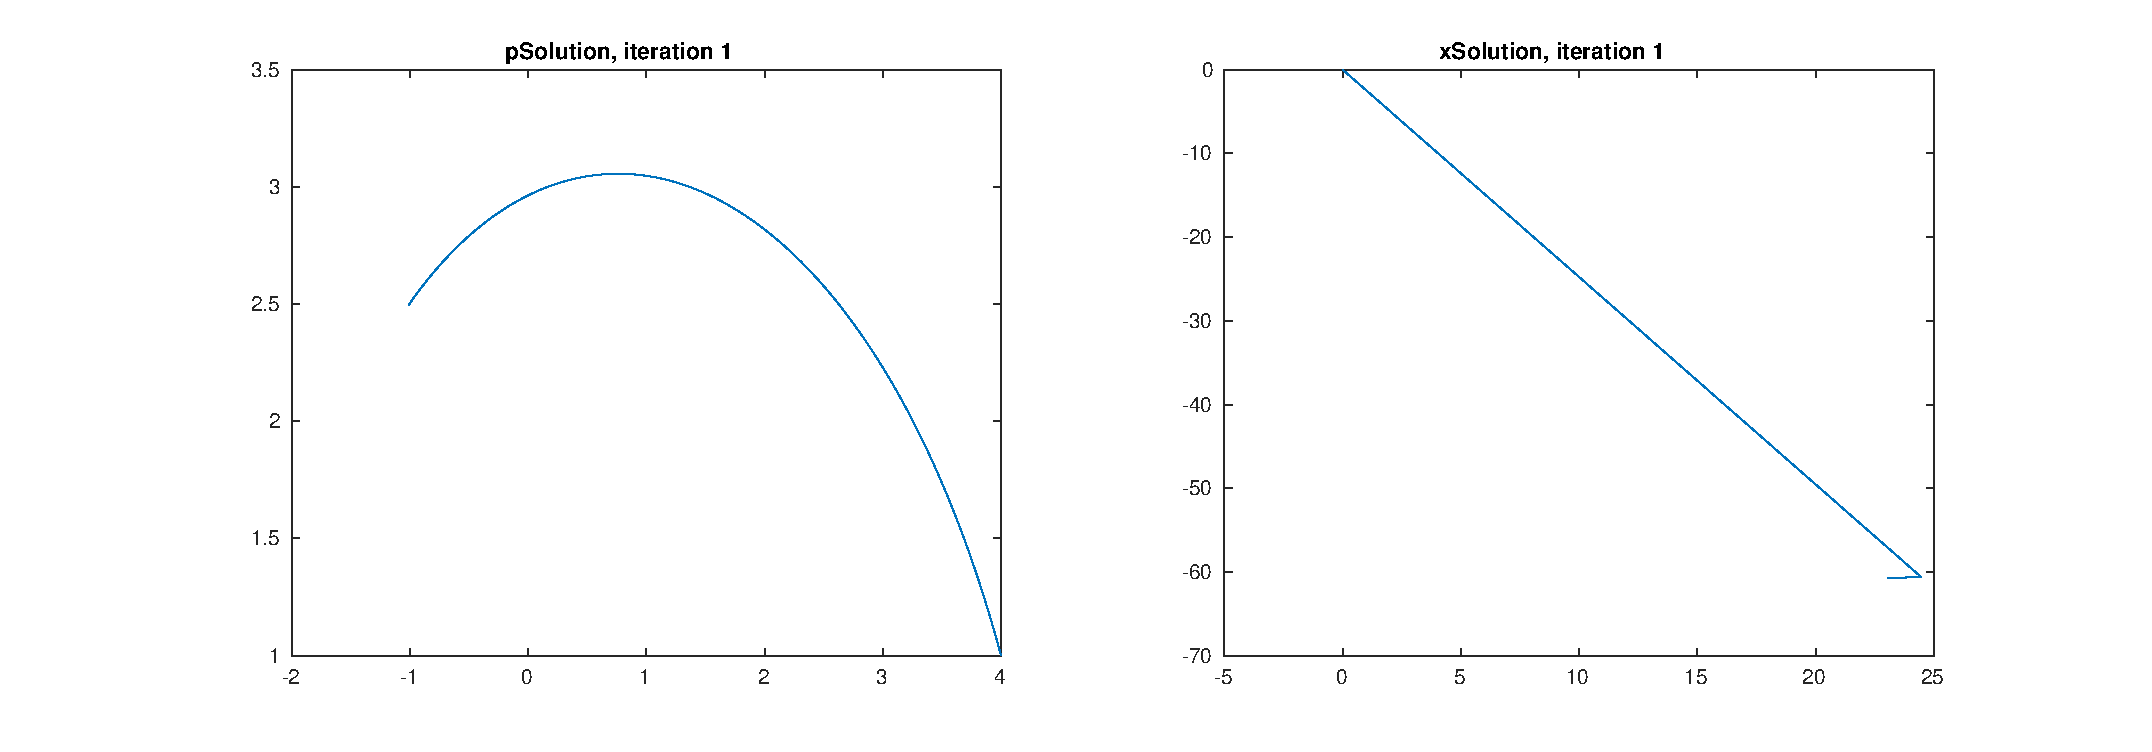
\includegraphics[width=\textwidth]{part2-failure}
	\caption{Failure when using iterative method directly}
	\label{fig:p2-failure}
\end{figure}
\section{A maybe reason}
The failure arises from the fact that when $x$ starts from $0$, so as $b(x)$.
We can observe from the first equation
$$ x' = \frac{C}{|b|_a}(ap+b) $$
that $(ap+b)$ is supposed to be very near to $0$, which can hardly be satisfied in the first iterative round.
So $\frac{dx}{ds}$ gets very big in the first two iteration rounds, and the situation doesn't get better in the following rounds.
To avoid such problem, we give an alternative way to solve the equation.

\part{Improvement based on a naive idea}
\section{Result of the improved method}
Since $\frac{dx}{ds}$ have singularity at $x=0$ if $p$ is not enough small, a simple improvement comes up very naturally: the initial condition varies in every iteration round, but it will converge to the stable point (int this case $(0, 0)^T$).
Specifically, we use the following border condition:
\begin{align}
	p(0) &= (4, 1)^T \\
	x^{(k)}(1) &= (0, 0)^T + (1/k, 0)^T
\end{align}
here $k$ denotes the iteration round.
The form of the converging initial points is not so important, since only its converging rate matters.

The following chart shows how the improved method works.
\begin{figure}[h]
	\centering
	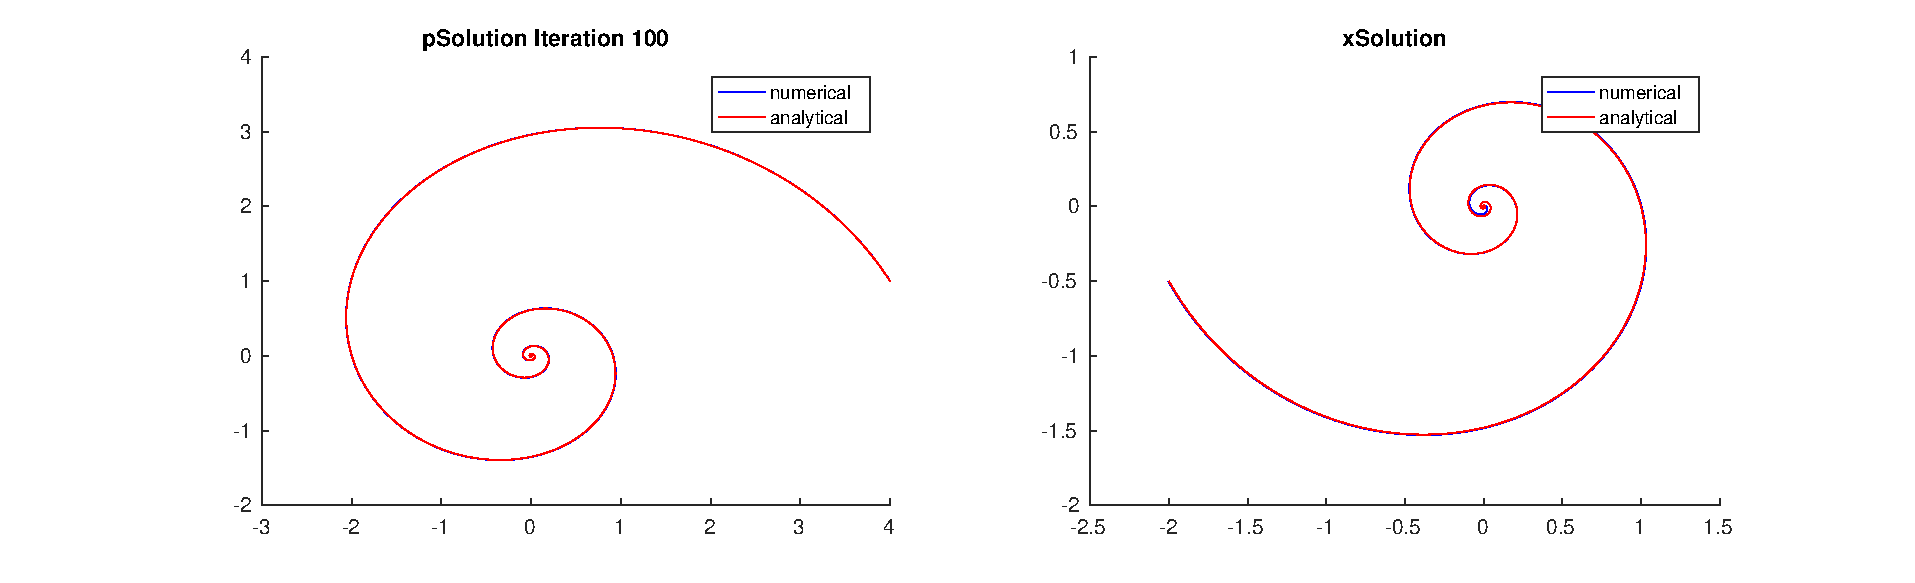
\includegraphics[width=\textwidth]{part3-demo}
	\caption{A demonstration of varing initial condition method}
	\label{fig:p3-demo}
\end{figure}
\begin{figure}[h]
	\centering
	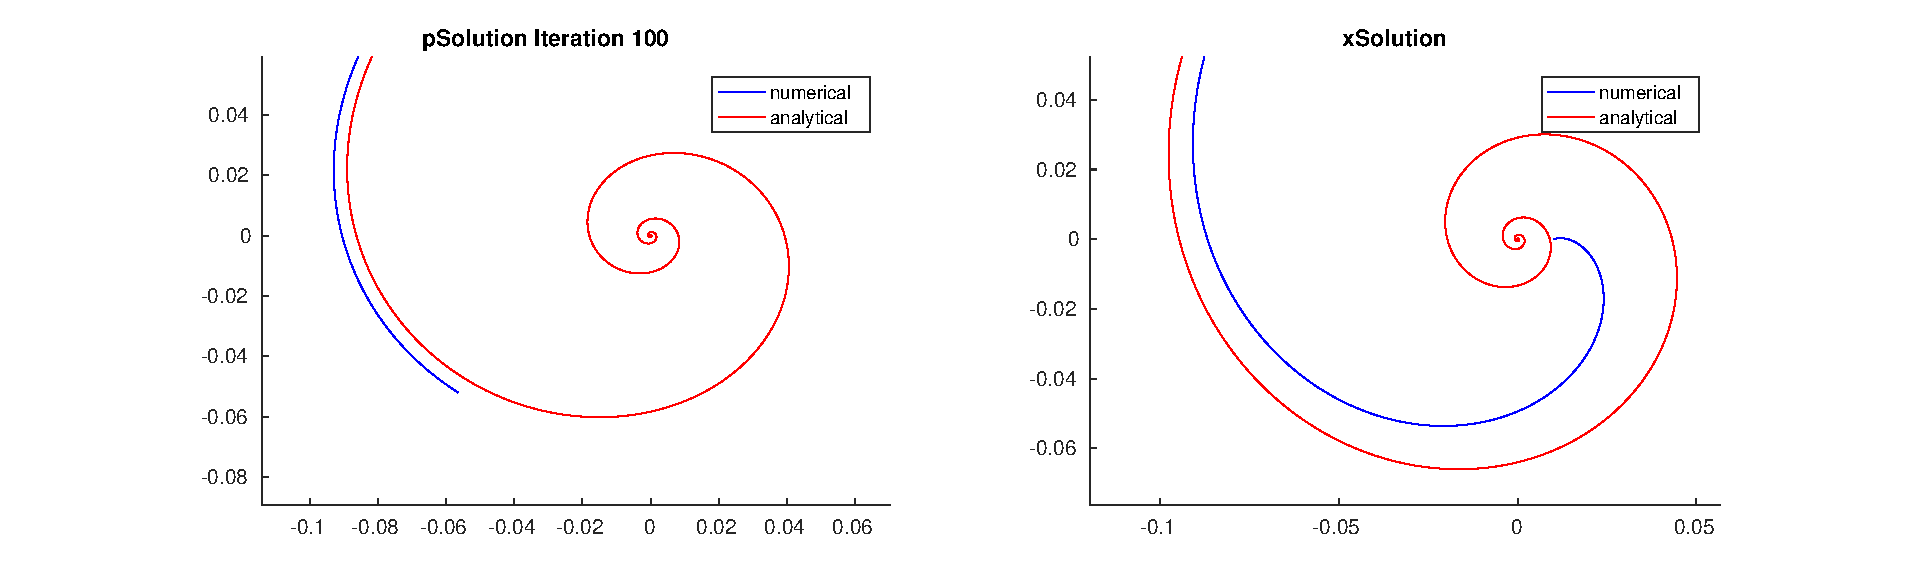
\includegraphics[width=\textwidth]{part3-demo-zoomin}
	\caption{A close lookup near the stable point}
	\label{fig:p3-demo-zoomin}
\end{figure}

The two figures lead to some interesting conculsions:
\begin{enumerate}
	\item As the initial condition is far from the final result, the iterative method still works (but that may largely depends on the fineness of the equations).
	\item The error of the $p$ part increases steadily as the length $s$, while the error of $x$ is much larger.
	\item Notice that we set the termination condition as $||p^{(k+1)} - p^{(k)}|| < criterion = 10^{-6}$, but the actual error is about $5 \times 10^{-3}$, not at the same magnitude (see figure \ref{fig:p3-demo-pEnd}). A similar situation happens at the $x$ side.
\end{enumerate}
\begin{figure}[h]
	\centering
	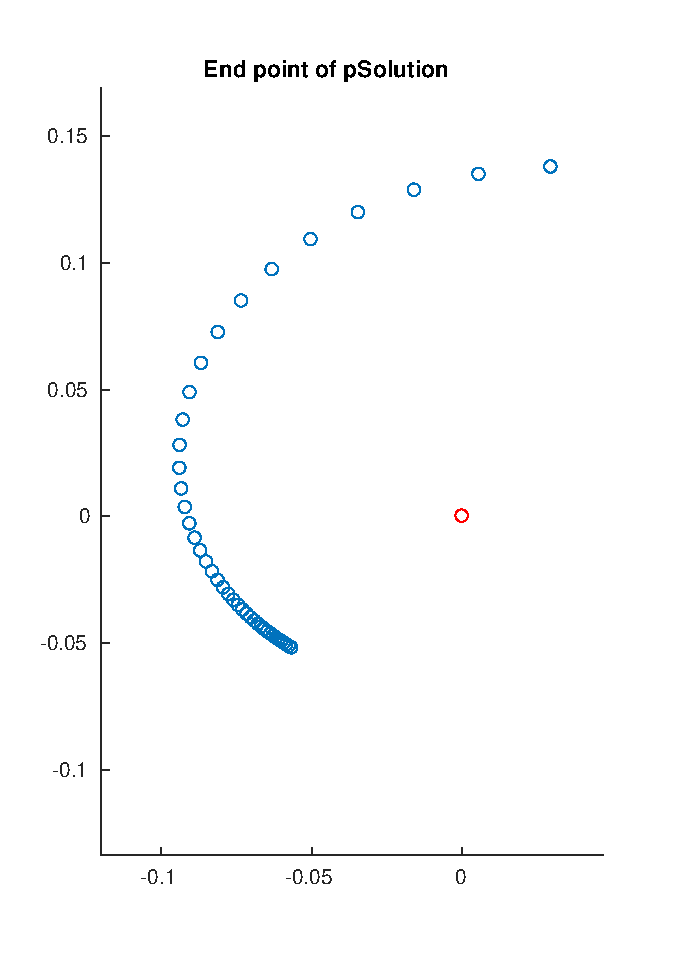
\includegraphics[width=0.5\textwidth]{part3-demo-pEnd}
	\caption{$p(1)$ spires in and converges very slowly}
	\label{fig:p3-demo-pEnd}
\end{figure}

\section{An attempt on quicker convergence}
\label{sec:attempt-qc}
We should notice that in the border condition mentioned before, the convergence rate is rather low; in fact, it will nearly stop if the iteration goes on.
So a very natural idea is if we can `speed up' the iteration by choosing a faster converging initial condition: $$ x^{(k)}(1) = max\{2^{(1-k)}, 1/resolution\}. $$
The intermediate result at 18th iteration shows in figure \ref{fig:p3-try-quick-convergence}.
\begin{figure}[h]
	\centering
	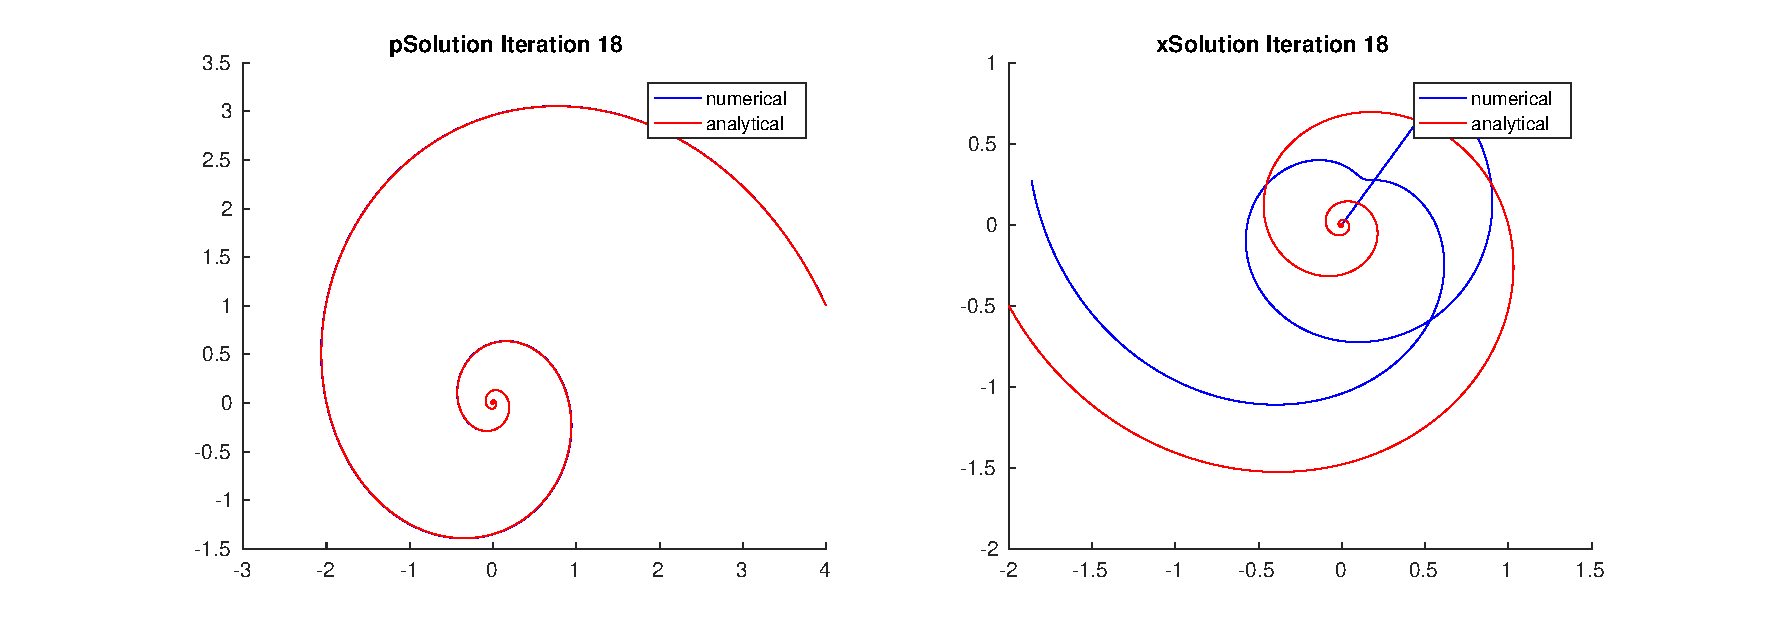
\includegraphics[width=\textwidth]{part3-try-quick-convergence}
	\caption{An unsuccessful example of speed up convergence}
	\label{fig:p3-try-quick-convergence}
\end{figure}

The main problem lies in that the solution has no time to converge before the initial condition gets too small, so we have the following improvement.

\section{Criterion selection}
Before we carry out any numerical experiment, the criterion of convergence should be carefully taken.
Here we test over criterions with different orders.
It is clear that $10/resolution$ is quite enough for precision, and $0.1/resolution$ may be a better choice.
\begin{figure}[h]
	\centering
	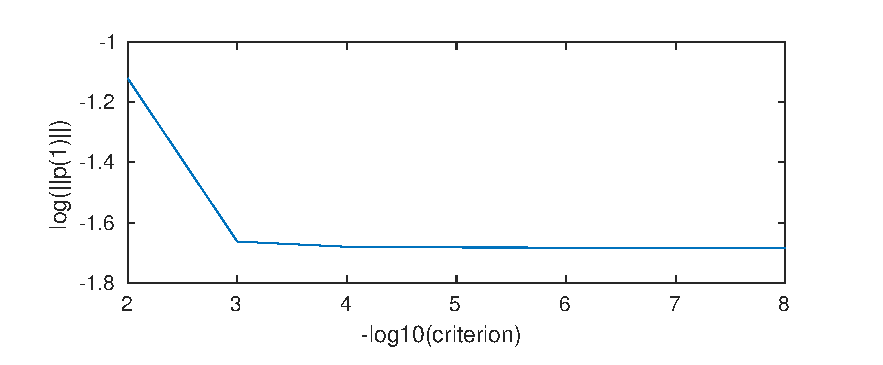
\includegraphics[width=0.7\textwidth]{part3-error-with-criterion}
	\caption{Error in $p$ under different criterion conditions, $resolution = 10^4$}
	\label{fig:p3-error-with-criterion}
\end{figure}

\section{An improvement on initial condition}
Since in section \ref{sec:attempt-qc} we have found that the solution diverges because the initial condition converges too quicklly, we can `wait' for the solution to converge before the initial condition get closer to the stable point.
To write it explicitly, we have
\begin{equation}
	x^{(k+1)}(1) = 
	\begin{cases}
		x^{(k)}(1) / 2 & if \quad ||p^{(k+1)}(1) - p^{(k)}(1)|| < criterion \\
		x^{(k)}(1) & otherwise
	\end{cases}
\end{equation}
Four cases are tested, where $resolution \in \{10^3, 10^4, 10^5, 10^6\}$, with $criterion = 0.1 / resolution$.
\begin{figure}[h]
	\centering
	\subfigure[Error of $p(1)$]{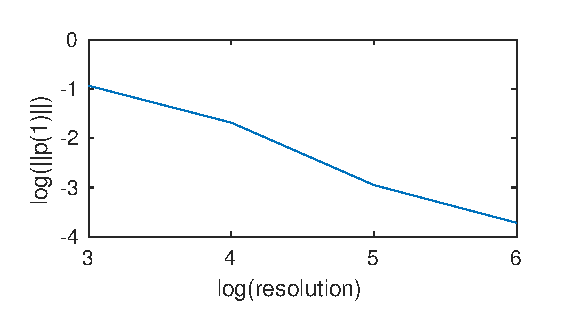
\includegraphics[width=0.4\textwidth]{part3-improved-solution-error}}
	\subfigure[Error of $p(1)+(B+B^T)x(1)$ in phase space]{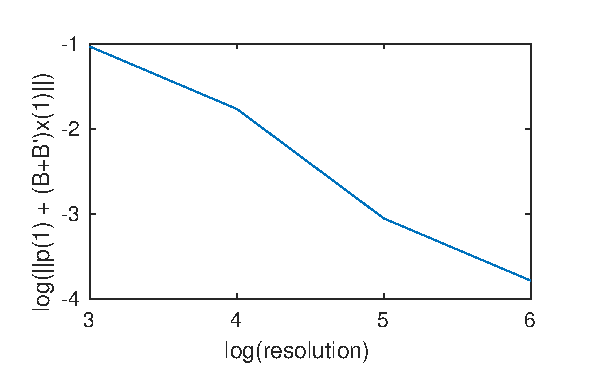
\includegraphics[width=0.4\textwidth]{part3-improved-phase-space-error}}
	\label{fig:p3-improved-solution}
\end{figure}

As figure \ref{fig:p3-improved-solution} shows, error of numerical solution (measured by $||p(1)||$) is indeed in first order.
If we measure the error in phase space (I wonder if it is more important), the result is shown in the figure, similar as the previous result.

It may be quite interesting to have a look at how long these iterations take, in terms of round numbers.
Results are shown in table \ref{tab:p3-iterations}.
It is intriguing that every even initial condition round has just one iteration.
It seems that it takes exponentially time as the resolution increases.

\begin{table}[h]
	\centering
	\caption{Iterations used}
	\label{tab:p3-iterations}
	\begin{tabular}{c|cccc}
		\hline
		\multirow{2}{*}{log2($x^{(k)}(1)$)} & \multicolumn{4}{c}{Resolution}\\
		& $10^3$& $10^4$& $10^5$& $10^6$\emph{($criterion=10^{-6}$)}\\
		\hline
		$0$& 14& 17& 19& 19\\
		$-1$& 1& 1& 1& 1\\
		$-2$& 15& 19& 23& 23\\
		$-3$& 1& 1& 1& 1\\
		$-4$& 39& 45& 52& 52\\
		$-5$& 1& 1& 1& 1\\
		$-6$& 74& 76& 87& 87\\
		$-7$& 0& 1& 1& 1\\
		$-8$& 0& 105& 126& 126\\
		$-9$& 0& 1& 1& 1\\
		$-10$& 0& 0& 154& 163\\
		$-11$& 0& 0& 1& 1\\
		$-12$& 0& 0& 186& 202\\
		$-13$& 0& 0& 1& 1\\
		$-14$& 0& 0& 0& 7\\
		$-15$& 0& 0& 0& 203\\
		$-16$& 0& 0& 0& 1\\
		\hline
	\end{tabular}
\end{table}

\part{Further more}
\section{Using high-order schemes}
Since the convergence is in first order, we wonder if the method can converge much faster with high-order schemes.
However, according to result shown in figure \ref{fig:p3-improved-hsolution-error}, if we use improved Euler method in each iteration round, the convergence rate is still in first order.
\begin{figure}[h]
	\centering
	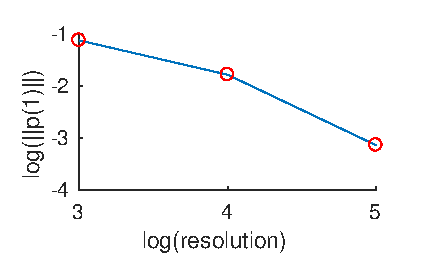
\includegraphics[width=0.4\textwidth]{part3-improved-hsolution-error}
	\caption{Error of $p(1)$, with each iteration using improved Euler method}
	\label{fig:p3-improved-hsolution-error}
\end{figure}

\section{Tests on higher-order equations}
A random normal matrix is chosen to test if the method is robust in higher dimension cases.
Here, we select $B$ to be
$$
\begin{bmatrix}
-0.9456 & 0.4262 & 0.2393 \\
0.4262 & -0.9631 & -0.0686 \\
0.2393 & -0.0686 & -1.0911 \\
\end{bmatrix}
$$
which has three real eigenvalues.
The resulting is quite confusing, because convergence emerges after at most 1300 rounds, when resolution is set to be $10^5$.
However, the result of $resolution=10^3, 10^4$ is to satisfactory; see figure \ref{fig:p3-newB}
\begin{figure}[h]
	\centering
	\subfigure[Error of $p(1)$]{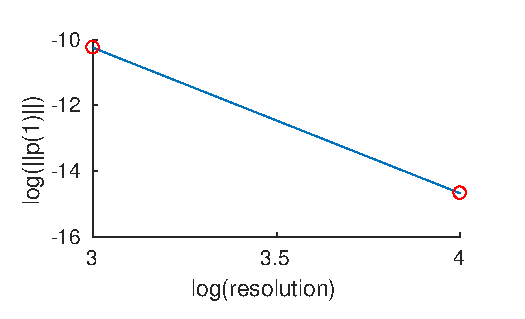
\includegraphics[width=0.4\textwidth]{part3-newB-s}}
	\subfigure[Error of $p(1)+(B+B^T)x(1)$ in phase space]{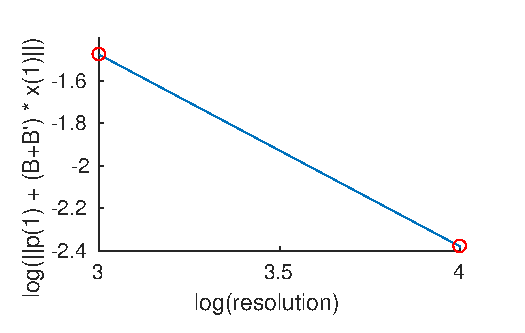
\includegraphics[width=0.4\textwidth]{part3-newB-p}}
	\label{fig:p3-newB}
\end{figure}
\end{document}
